\documentclass[a4paper,14pt]{extarticle}
\usepackage{../../tex-shared/report-layout}

\renewcommand{\mylabnumber}{2}
\renewcommand{\mylabtitle}{Корреляционный и регрессионный анализ данных}
\renewcommand{\mysubject}{Интеллектуальный анализ данных}
\renewcommand{\mylecturer}{Сырых О.А.}

\begin{document}
\begin{titlepage}
    
    \thispagestyle{empty}
    
    \begin{center}
        
        Министерство науки и Высшего образования Российской Федерации \\
        Севастопольский государственный университет \\
        Кафедра ИС
        
        \vfill

        Отчет \\
        по лабораторной работе №\mylabnumber \\
        \enquote{\mylabtitle} \\
        по дисциплине \\
        \enquote{\MakeTextUppercase{\mysubject}}

    \end{center}

    \vspace{1cm}

    \noindent\hspace{7.5cm} Выполнил студент группы ИС/б-17-2-о \\
    \null\hspace{7.5cm} Горбенко К. Н. \\
    \null\hspace{7.5cm} Проверил \\
    \null\hspace{7.5cm} \mylecturer

    \vfill

    \begin{center}
        Севастополь \\
        \the\year{}
    \end{center}

\end{titlepage}

\section{Цель работы}
\begin{itemize}
    \item исследовать возможности языка R для проведения корреляционного и регрессионного анализа данных;
    \item создание набора данных для проведения корреляционного и регрессионного анализа данных.
\end{itemize}

\section{Задание на работу}
\begin{enumerate}
    \item Исследовать основные функции и команды языка R, представленные в
          данной лабораторной работе;
    \item выполнить все примеры;
    \item подобрать экспериментальные данные для анализа;
    \item выполнить ввод данных с клавиатуры;
    \item провести экспорт данных из текстового файла с разделителями;
    \item выполнить экспорт данных из Excel.
\end{enumerate}

\section{Ход работы}
\subsection{Ввод данных}
Выполним ввод данных с клавиатуры:
\begin{lstlisting}
> data <- data.frame(country=character(0), totalCasesBy1m=numeric(0), deathBy1m=numeric(0), testsBy1m=numeric(0), healthIndex=numeric(0), stringencyIndex=numeric(0))
> data <- edit(data)
\end{lstlisting}
Результат выполнения программы приведен на рисунке \ref{fig:edit}.
\begin{figure}[H]
    \centering
    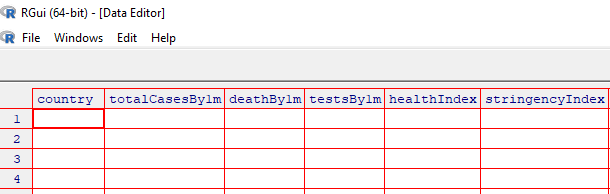
\includegraphics[width=\linewidth]{edit}
    \caption{Ввод данных с клавиатуры}
    \label{fig:edit}
\end{figure}

Выполним ввод данных из текстового файла:
\begin{lstlisting}
> data <- read.table("D:\\Repositories\\Learning\\ИАД\\data.csv", header=TRUE, sep=",")
> data
\end{lstlisting}
Результат выполнения программы приведен на рисунке \ref{fig:csv}.
\begin{figure}[H]
    \centering
    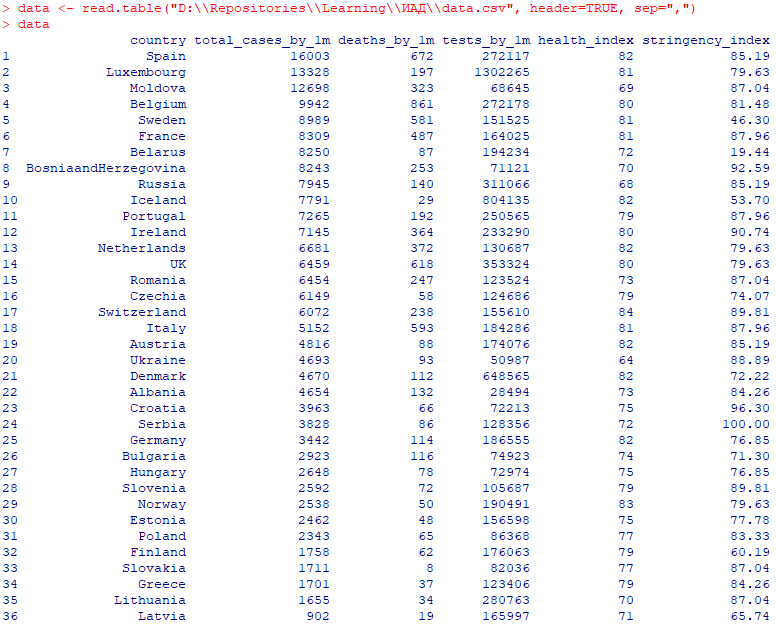
\includegraphics[width=\linewidth]{from-csv}
    \caption{Ввод данных из .csv файла}
    \label{fig:csv}
\end{figure}

Выполним ввод из xlsx файла:
\begin{lstlisting}
library("xlsx")
> data <- read.xlsx("D:\\Repositories\\Learning\\ИАД\\data.xlsx", 1)
> data
\end{lstlisting}
Результат выполнения программы приведен на рисунке \ref{fig:xlsx}.
\begin{figure}[H]
    \centering
    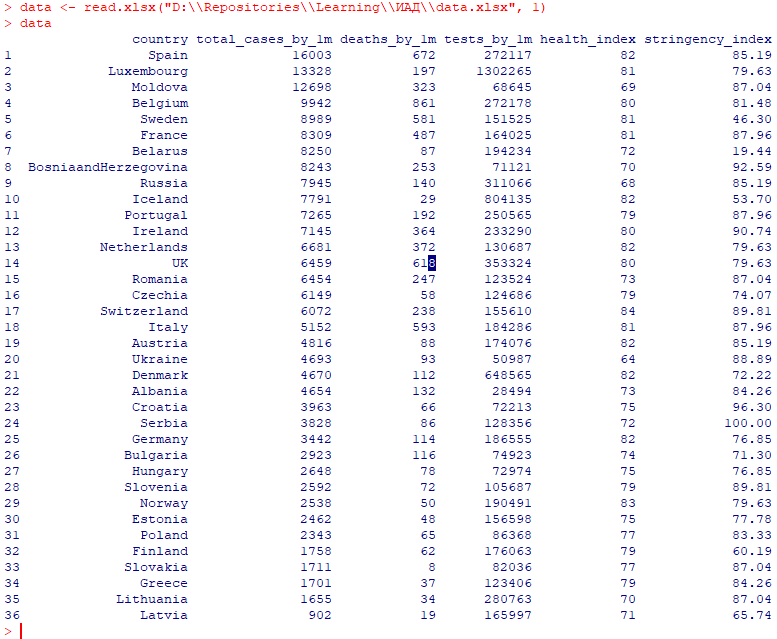
\includegraphics[width=\linewidth]{from-xlsx}
    \caption{Ввод данных из .xlsx файла}
    \label{fig:xlsx}
\end{figure}

\subsection{Построение графиков}
Выведем индекс строгости для нескольких стран:
\begin{lstlisting}
> countries <- data[[1]]
> indexes <- data[[6]]
> plot(factor(countries[1:5]), indexes[1:5], col="red", xlab="Country", ylab="Stringency Index", ylim=c(0, 100))
\end{lstlisting}
Результат выполнения программы приведен на рисунке \ref{fig:stringency}.
\begin{figure}[H]
    \centering
    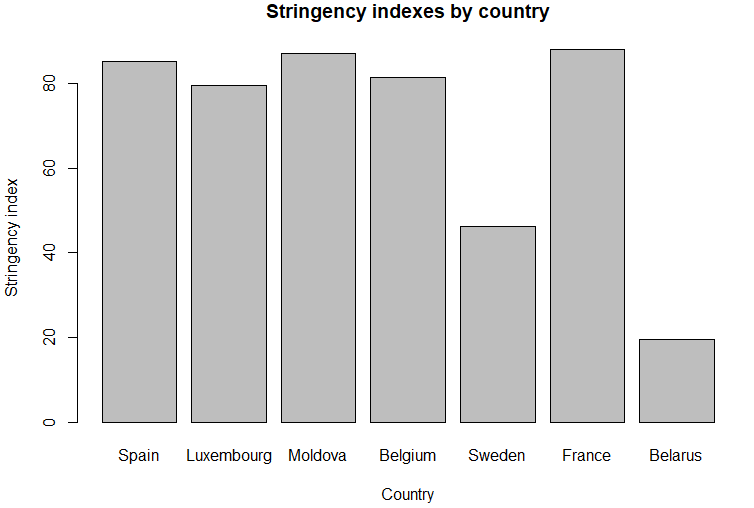
\includegraphics[width=.5\linewidth]{stringency}
    \caption{Индексы строгости стран}
    \label{fig:stringency}
\end{figure}

Выведем коэффициенты здравоохранения для всех стран:
\begin{lstlisting}
countries <- data[[1]]
healthIndexes = data[[5]]
library(ggplot2)
qplot(factor(countries),
      healthIndexes,
      geom="boxplot",
      xlab="Countries",
      ylab="Health indexes") +
    theme(axis.text.x=element_text(angle=90, vjust=0.5, hjust=1)) +
    geom_bar(stat="identity", position="stack") +
    labs(x=NULL, y="Health indexes")
\end{lstlisting}
Результат выполнения программы приведен на рисунке \ref{fig:stringency}.
\begin{figure}[H]
    \centering
    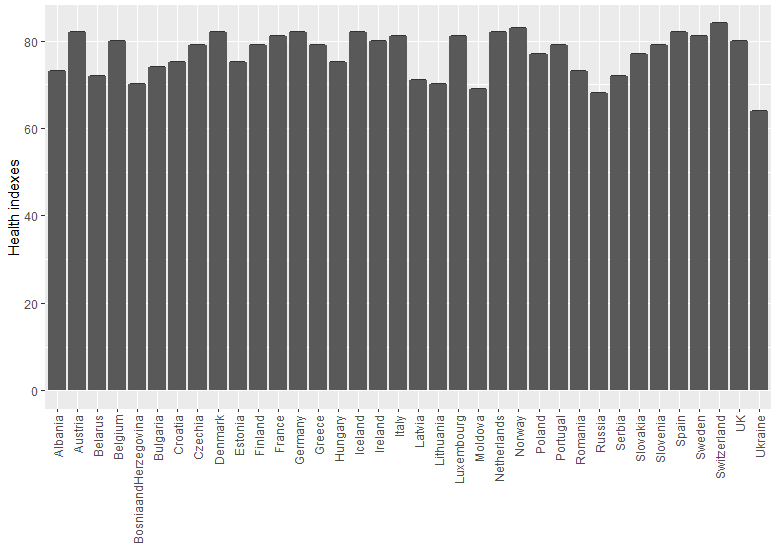
\includegraphics[width=\linewidth]{health-indexes}
    \caption{Коэффициенты здравоохранения стран}
    \label{fig:health-indexes}
\end{figure}

\subsection{Вычисление корреляции}
Вычислим матрицу корреляции методами Пирсона и Спирмена:
\begin{lstlisting}
cor(data[c("total_cases_by_1m", "deaths_by_1m", "tests_by_1m", "health_index", "stringency_index")],
    method="pearson",
    use="complete")

cor(data[c("total_cases_by_1m", "deaths_by_1m", "tests_by_1m", "health_index", "stringency_index")],
    method="spearman",
    use="complete")
\end{lstlisting}
Результат выполнения программы приведен на рисунке \ref{fig:cor}.
\begin{figure}[H]
    \centering
    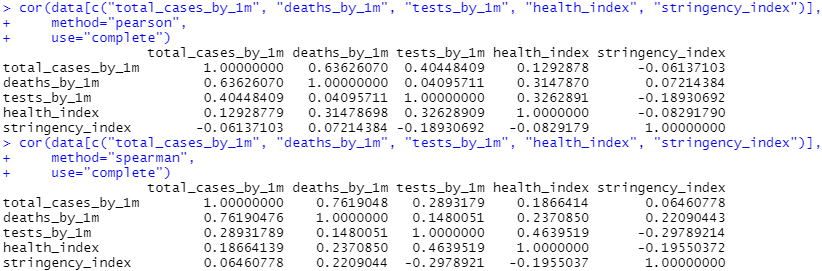
\includegraphics[width=\linewidth]{cor}
    \caption{Матрицы корреляции, составленные методами Пирсона и Спирмена}
    \label{fig:cor}
\end{figure}

Судя по коэффициентам, сильная корреляция наблюдается только между количеством
заражений и количеством смертей. Средняя - между количеством заражений и
количеством тестов, между количеством тестов и смертей и коэффициентами
здравоохранения. Во всех остальных случаях -- корреляция слабая.

Выполним оценку уровня значимости коэффициента корреляции между коэффициентами
здравоохранения и количеством смертей и между индексом строгости и количеством
заражений.
\begin{lstlisting}
with(data, cor.test(health_index, deaths_by_1m, method="pearson"))
with(data, cor.test(stringency_index, total_cases_by_1m, method="pearson"))
\end{lstlisting}
Результат выполнения программы приведен на рисунке \ref{fig:cor-level}.
\begin{figure}[H]
    \centering
    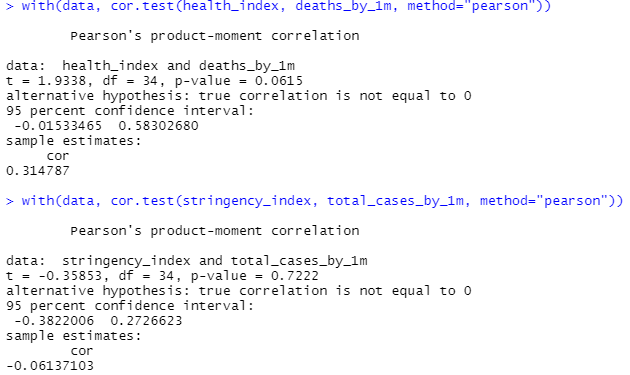
\includegraphics[width=.7\linewidth]{cor-level}
    \caption{Оценка уровня значимости коэффициента корреляции}
    \label{fig:cor-level}
\end{figure}

Для обоих случает связь между переменными не доказана, нулевая гипотеза не
отвергается.

Построим матрицу точечных графиков:
\begin{lstlisting}
scatterplotMatrix(~deaths_by_1m+health_index+stringency_index+tests_by_1m+total_cases_by_1m,
                  regLine=FALSE, smooth=FALSE, diagonal=list(method="density"), data=Dataset)
\end{lstlisting}
Результат выполнения программы приведен на рисунке \ref{fig:scatterplot-matrix}.
\begin{figure}[H]
    \centering
    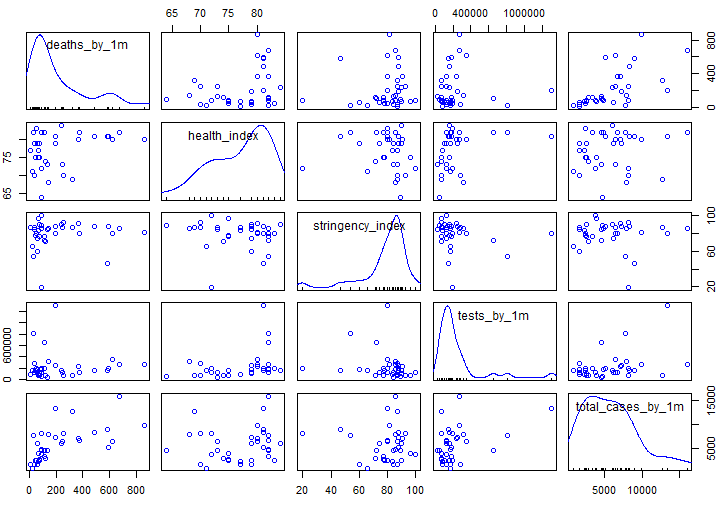
\includegraphics[width=\linewidth]{scatterplot-matrix}
    \caption{Матрица точечных графиков}
    \label{fig:scatterplot-matrix}
\end{figure}
\pagebreak

Построим уравнение зависимости количества смертей от индекса здравоохранения.
Получим функцию: $health\_index = 75.492 + 0.007 * death\_by\_1m$. Построим
график остатков.
\begin{figure}[H]
    \centering
    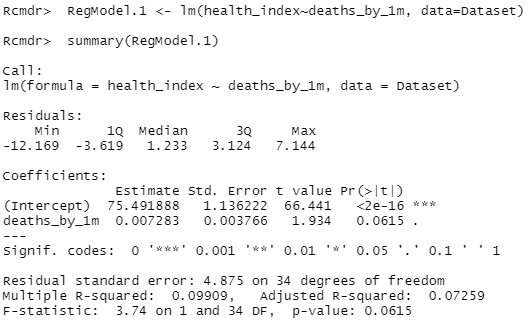
\includegraphics[width=.6\linewidth]{health-death-dependency-func}
    \caption{Уравнение зависимости индекса здравоохранения от количества смертей}
    \label{fig:health-death-dependency-func}
\end{figure}

\begin{figure}[H]
    \centering
    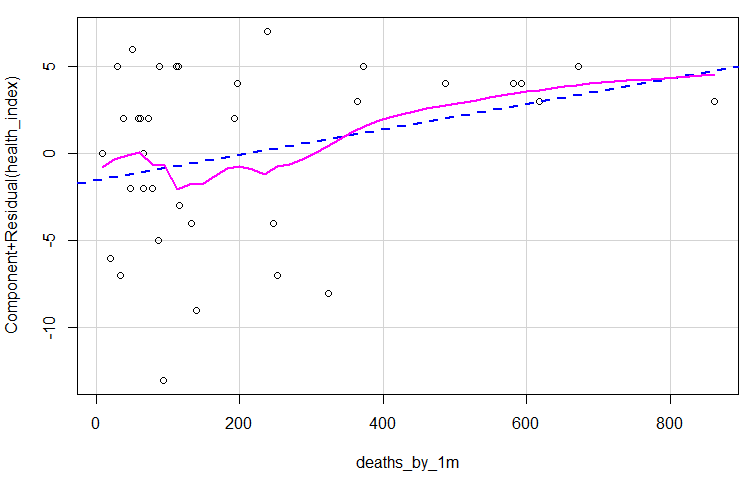
\includegraphics[width=.6\linewidth]{health-death-dependency-graph}
    \caption{График остатков для зависимости индекса здравоохранения от количества смертей}
    \label{fig:health-death-dependency-graph}
\end{figure}
Наблюдается прямая умеренная зависимость индекса здравоохранения от количества
смертей. Коэффициент корреляции Пирсона для этой связи выше коэффициента
корреляции Спирмена.

\pagebreak

Построим уравнение зависимости количества заражений от индекса
строгости. Получим функцию: $total\_cases = 6869.94 - 14.38 * stringency\_index$.
Построим график остатков.
\begin{figure}[H]
    \centering
    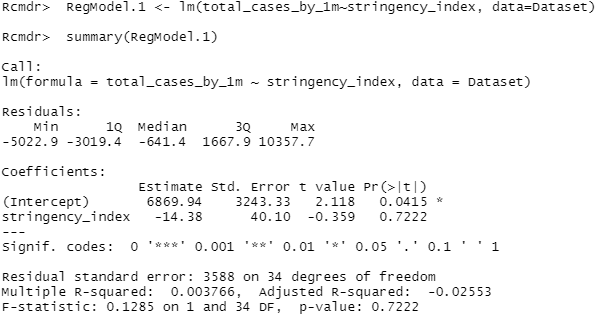
\includegraphics[width=.6\linewidth]{total-cases-stringency-func}
    \caption{Уравнение зависимости количества заражений от индекса строгости}
    \label{fig:total-cases-stringency-func}
\end{figure}

\begin{figure}[H]
    \centering
    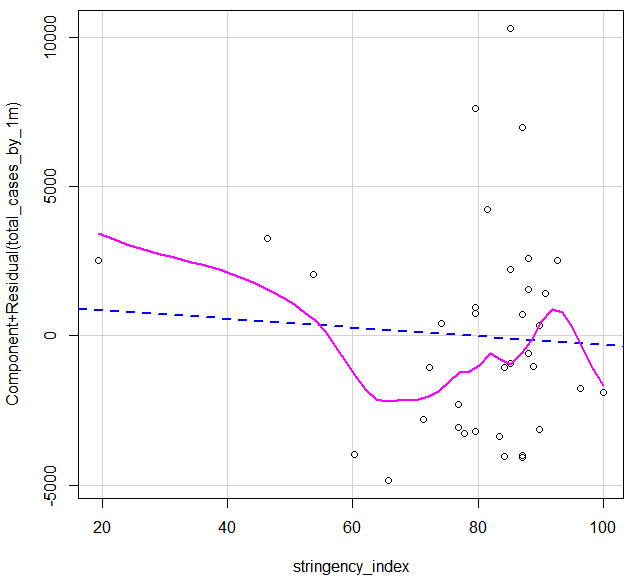
\includegraphics[width=.6\linewidth]{total-cases-stringency-graph}
    \caption{График остатков для зависимости количества заражений от индекса строгости}
    \label{fig:total-cases-stringency-graph}
\end{figure}
Коэффициент корреляции Пирсона для данной связи положителен, коэффициент
корреляции Спирмена -- отрицателен, что говорит о слабой связи между переменными
(или отсутствии связи). По модулю коэффициенты Пирсона и Спирмена отличаются на
0.003.
\pagebreak

Построим уравнение зависимости количества проведенных тестов от индекса
здравоохранения. Получим функцию $total\_tests = -973681 + 15516 *
health\_index$. Построим график остатков.
\begin{figure}[H]
    \centering
    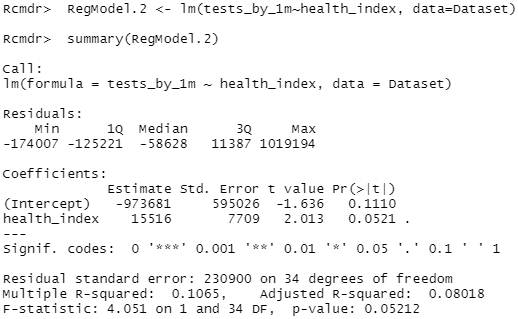
\includegraphics[width=.6\linewidth]{total-tests-health-func}
    \caption{Уравнение зависимости количества проведенных тестов от индекса здравоохрания}
    \label{fig:total-tests-health-func}
\end{figure}

\begin{figure}[H]
    \centering
    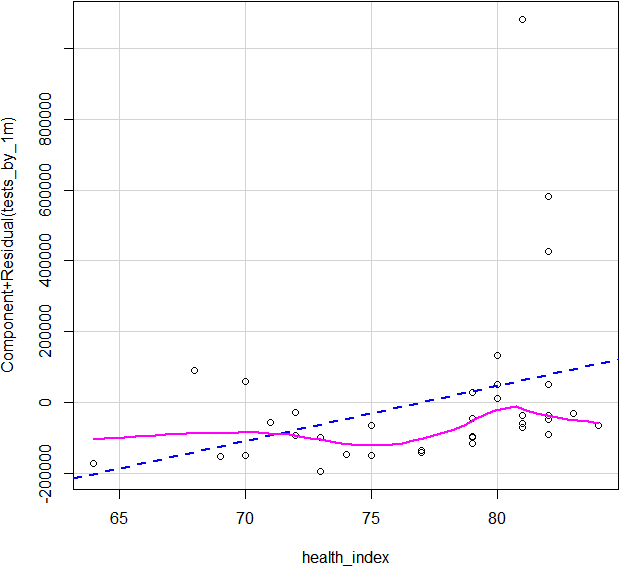
\includegraphics[width=.58\linewidth]{total-tests-health-graph}
    \caption{График остатков для зависимости проведенных тестов от индекса здравоохрания}
    \label{fig:total-tests-health-graph}
\end{figure}
Наблюдается прямая умеренная зависимость количества проведенных тестов от
индекса здравоохрания. Коэффициент корреляции Спирмена для данной связи выше,
чем коэффициент Пирсона.
\pagebreak

Построим уравнение множественной регрессии: $total\_death = -1206.777 + 14.757 *
health\_index + 1.138 * stringency\_index + 0.046 * total\_cases$
\begin{figure}[H]
    \centering
    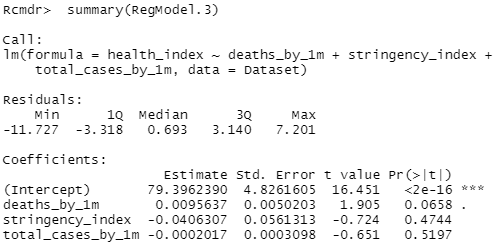
\includegraphics[width=.75\linewidth]{multi-reg}
    \caption{Уравнение множественной регрессии}
    \label{fig:multi-reg}
\end{figure}

Построим график компонента-остаток для модели множественной регрессии:
\begin{figure}[H]
    \centering
    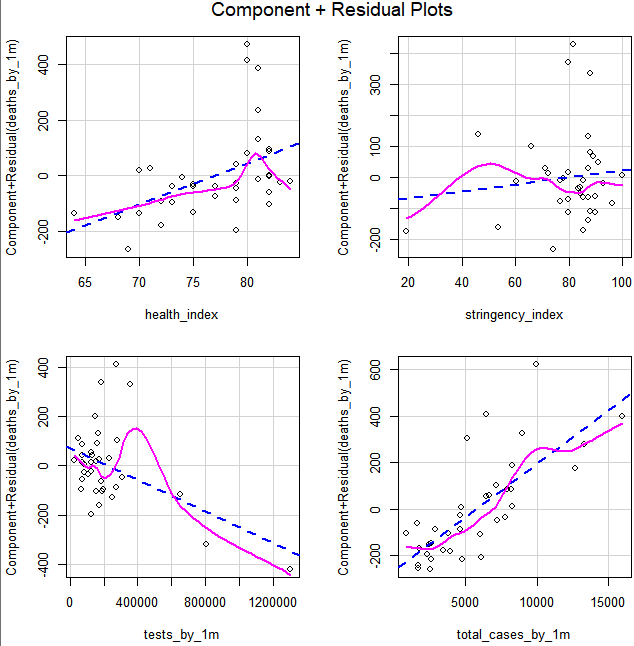
\includegraphics[width=.6\linewidth]{multi-reg-graph}
    \caption{Графики для модели множественной регрессии}
    \label{fig:multi-reg-graph}
\end{figure}

Построение регрессии по направлению вперед:
\begin{figure}[H]
    \centering
    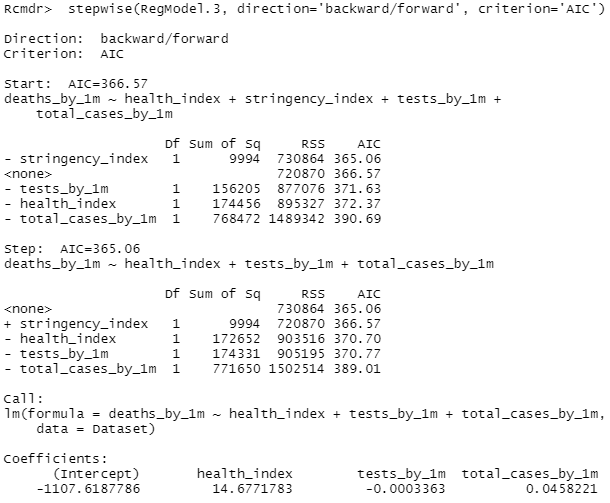
\includegraphics[width=.7\linewidth]{aic-forward}
    \caption{Пошаговое построение регрессии по направлению вперед}
    \label{fig:aic-forward}
\end{figure}
\pagebreak

Построение регрессии по направлению назад:
\begin{figure}[H]
    \centering
    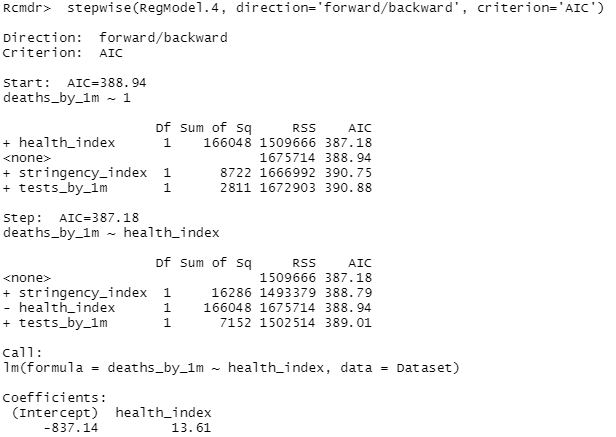
\includegraphics[width=.7\linewidth]{aic-backward}
    \caption{Пошаговое построение регрессии по направлению назад}
    \label{fig:aic-backward}
\end{figure}

Из построенных моделей можно сделать вывод, что модель, построенная по
направлению вперед, более предпочтительна, т.к. коэффициент AIC для нее
меньше. Уравнение: $total\_death = -1107.619 + 14.677 *
health\_index + 0.046 * total\_cases$.
\pagebreak

Проверим коэффициент VIF:
\begin{figure}[H]
    \centering
    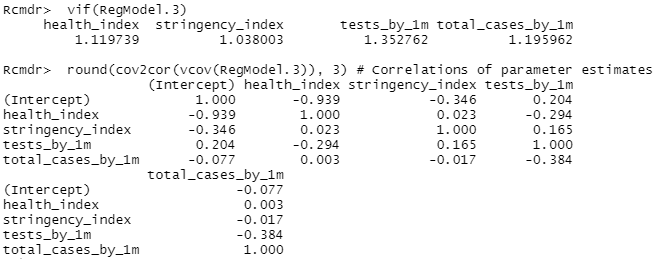
\includegraphics[width=.8\linewidth]{vif}
    \caption{Получение коэффициента VIF}
    \label{fig:vif}
\end{figure}

Так как значения коэффициента VIF меньше 10, мы можем сделать вывод о том, что
мультиколлинеарность отсутствует.

\section*{Выводы}
В ходе выполнения лабораторной работы были изучены такие типы данных в языке R,
как список, таблица. Также были изучены методы импорта текстовых файлов с
разделителями и Excel-файлов. Кроме того, были проанализированы зависимости между
переменными методами корреляции и регрессии.

Выяснилось, что количество смертей сильно коррелирует с количеством заражений,
количество заражений умеренно коррелирует с количество тестов, индекс здравоохранения
умеренно коррелирует с количеством смертей и количеством тестов.

Количество смертей сильно зависит от индекса здравоохранения.

\end{document}